\section{CMS-CL (CMS Configuration Language)}\label{CMS-CL}		
'CMS-CL' is a DSL. A DSL\cite{dslDefine} is a computer language for a specific domain (e.g. SQL, HTML, OCL, ...) : its syntax are designed to work in the targeted domain as good as possible. This syntax is composed of three parts : the \textit{abstract syntax} is the unvariable part (i.e. the structure of the language) without any particular representation. The \textit{semantics part} is about the meaning of the elements, and the \textit{concrete syntax} concerns the variable part, which describes the representation of the language. 
In the following sections, the CMS-CL syntaxs and semantics are detailed.		
			
			\subsection{CMS-CL Abstract Syntax and Semantics}\label{abstractSyntax} 
The DSL created for the website management contains several features allowing configuration modifications and creations by users. These elements have been represented in a metamodel~\cite{metaExplanation}: for the sake of conciseness, we do not show the entire metamodel\footnote{\scriptsize{CMS-CL complete metamodel: \url{https://raw.github.com/mallon/WordPress-MindMapping/master/Documentation/DetailedFigures/WdpDslCompleteMM.pdf}}}, but a simplified one in Fig.\ref{CMS-CLMetamodel}.
				\begin{figure}[!h]
					\centering
					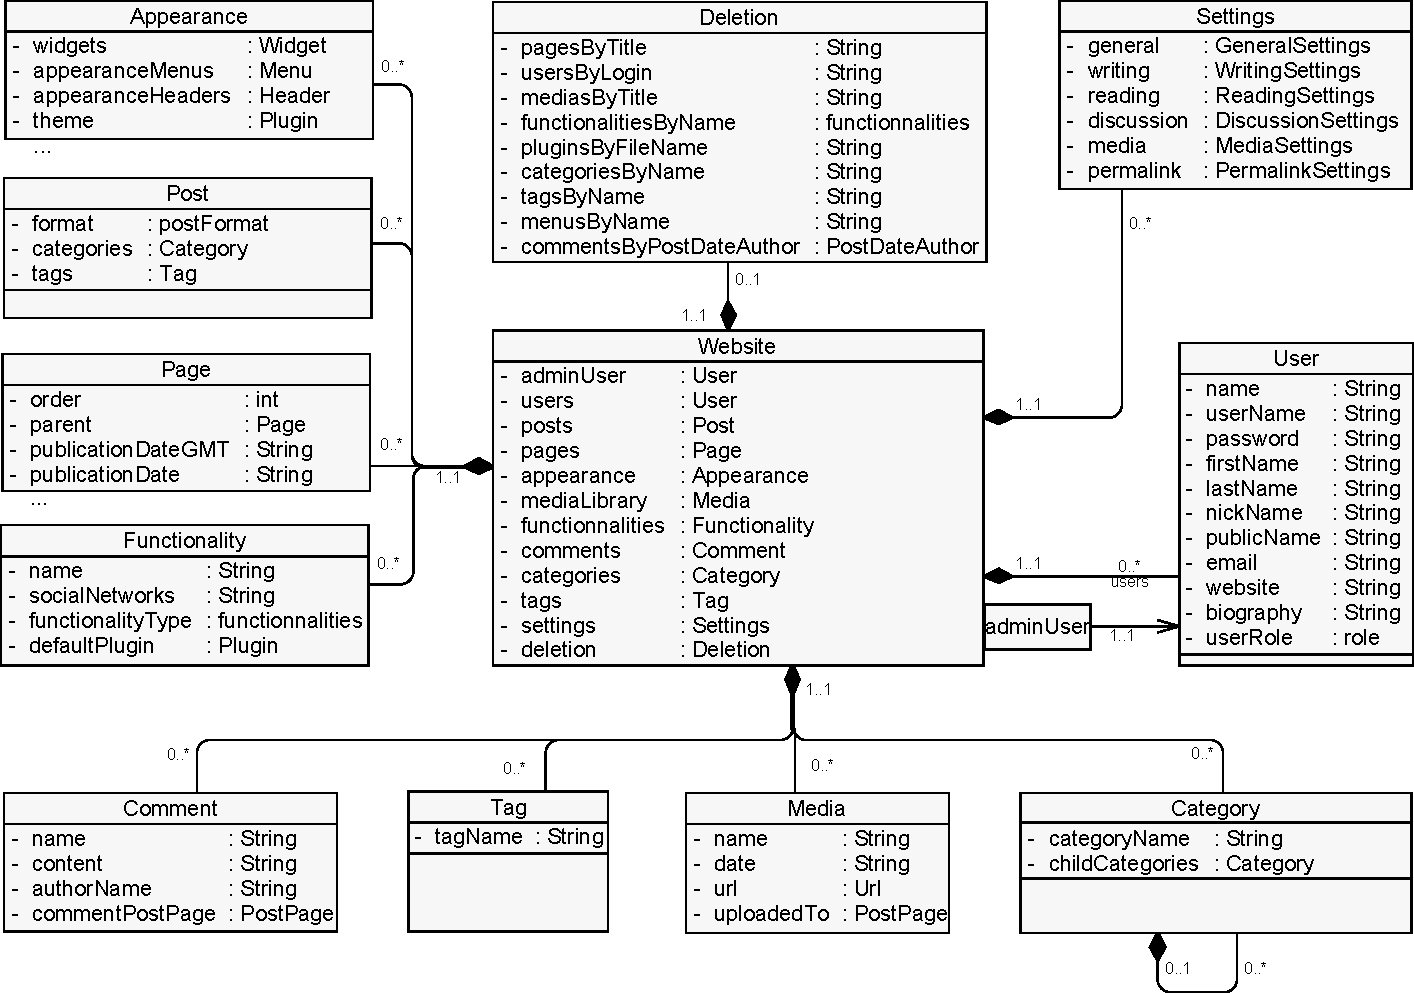
\includegraphics[width=\textwidth]{../resources/pdf/WOCMMSimplified.pdf}
					\caption{CMS-CL simplified metamodel (abstract syntax)}
					\label{CMS-CLMetamodel}
				\end{figure}	
							 								
\vspace{0.15em}
\noindent\textbf{User. \label{userElement}} With this concept, it is possible to create users with their mandatory respective roles (granting rights to the various elements of the site) : \textit{'Administrator', 'Editor', 'Author', 'Contributor' and 'Suscriber'}. It is important to notice that users modifying the website configuration  must have an administrator role, which is represented by the element \textit{'AdminUser'} (by default the users are connected with the administrator account automatically created during the WordPress server installation).
 
\vspace{0.15em}
\noindent\textbf{Appearance.}End users will be able to change the appearance of the website, using the elements of 'Appearance'. The \textit{'apperanceHeader'} and \textit{'theme'} elements will respectively change the header of the site's main page and select a new theme. Its modification will influence how other features appear (e.g. the placement of the page on the website). For the 'Theme' feature, there are six default themes, choosen accordingly to the list of the most popular ones in 2013 \cite{topTheme} : \textit{Responsive, Magazine, Business, Galleries, Artistic and SEO}. 
The item \textit{'Menus'\label{menu}} allows changing the default content of the navigation elements. It is possible to change the default  access to the pages and posts, by creating a new item \textit{'Menu'} with external links (\textit{'Links'}), pages/posts categories (\textit{'Categories'}) or pages (\textit{'Accessed pages'}). 
Furthermore, end users can add functionalities to the site (and are displayed regardless of the page/post) with the twelve default \textit{'Widgets'}.

\vspace{0.15em}
\noindent\textbf{Deletion.} This entity contains all the names of the various items that the user wish to delete.

\vspace{0.15em}
\noindent\textbf{Comment.} It represents the comments write by users on a page/post.

\vspace{0.15em}
\noindent\textbf{Category.} Each categories can be composed in sub-categories. For instance, it can exists a category 'Music' containing two sub-categories 'Group' and 'Concert'.

\vspace{0.15em}
\noindent\textbf{Media.} This feature corresponds to images and videos which can be inserted with the content.

\vspace{0.15em}
\noindent\textbf{Tag.} It allows to find various posts concerning a same subject. Navigation within a website can be easy through the use of tags in order to find a particular information : for this reason, a tag can be added to a post.

\vspace{0.15em}
\noindent\textbf{Functionality.} Users usually wish to customize their web site according to their needs. Hence, a set of default functionalities is provided: \textit{eCommerce, spam, indexing, multilanguage, seo, pictures, and social Networks}. The users may select a functionality among them , or install another one ('plugin' attribute).

\vspace{0.15em}
\noindent\textbf{Page and Post.} Users (which have the correct rights) can add posts. Pages can be also added, and for this two elements, the author correspond to the administrator account of the user (see 'User' details \ref{userElement}). 

\vspace{0.15em}
\noindent\textbf{Settings.} 
It contains the various types of configuration : \textit{General, Writing, Reading, Media} and \textit{Permalinks}. In the \textit{GeneralSettings} class, \textit{login} and \textit{administrator} password attributes are required to enable the connection (to the platform site creation) which is realized with the platform \textit{address} attribute. But the settings require more technical knowledges, therefore the end-users will not have the possibility to modify it : only the web-designers will be able to do this (section \ref{webDesigners}).
				
			\subsection{CMS-CL Concrete Syntax}\label{concreteSyntax}	
			   	In the next two paragraphs, we present the tool used to represent a mind-map and the CMS-CL concrete 
			   	syntax, which is the visual representation. A mapping between the metamodel concepts (the abstract 
			   	syntax) and this visual representation (the mind-mapping) was necessary.
			   	
			   \vspace{0.15em}
			   \noindent\textbf{Representation Tool used.}\label{representationTools}
			   			There are a lot of different softwares for mind	mapping, and FreeMind was during a long time of those who
			   			have different interesting features : popularity, soundness, interactiveness, open 
			   			source, extensibility, export facilities and scripting. A fork of FreeMind was created: Freeplane. It 								provides and improves some of the 
			   			points mentioned above: a regularly updating and an improved extension system~\cite{freeplane}.
																	
				\vspace{0.15em}
				\noindent\textbf{CMS-CL and mind-mapping.} A mind-map is a diagram used to present concepts (or other items like tasks). There is one central governing concept, which is in the center of this 							diagram, and each other concepts are related to it. Each idea is symbolized as a child node of the central node (i.e. the central concept), and the 							various relations between these concepts are represented through edges. The software presented above adds the possiblity to create attributes for a 								node : an attribute is a node property (e.g. an address for a website).
									
						\begin{figure}[!h]
							\centering
							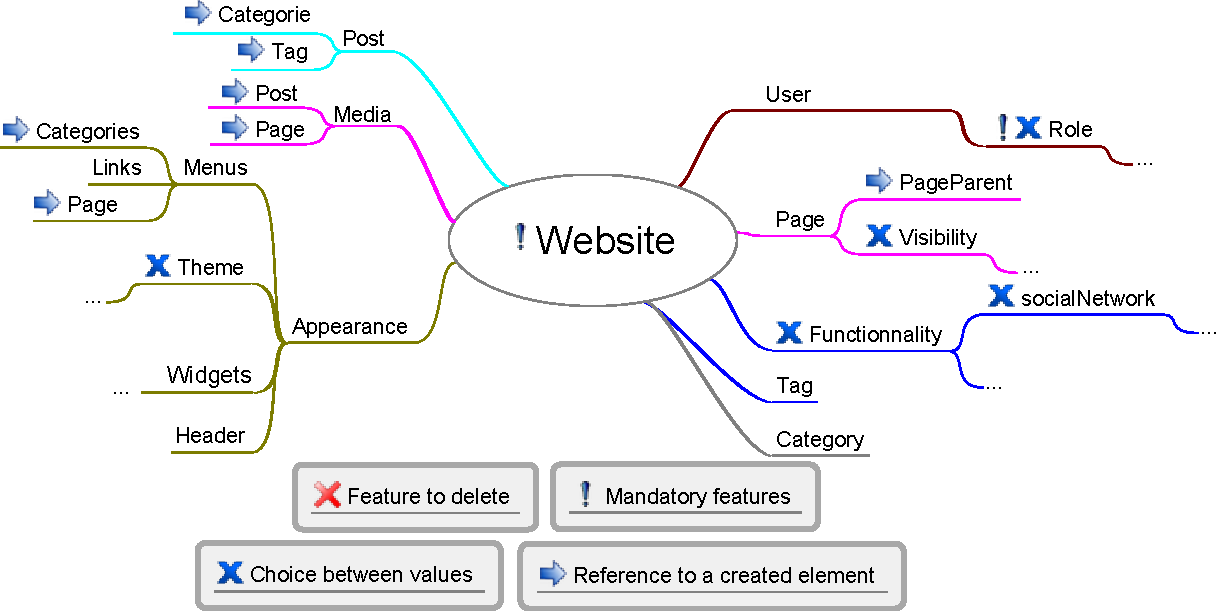
\includegraphics[width=0.85\textwidth]{../resources/pdf/CMS-CLFeatures.pdf}
							\caption{CMS-CL on top of the FreePlane metamodel (simplified representation)}
							\label{websiteDSLFeatures}
						\end{figure}
						The various concepts, their parameters and relationships are respectively represented by nodes, 
						attributes, and edges. CMS-CL has a visual representation via the mind mapping and it is on top of the Freeplane metamodel. 
						To adapt our DSL to this metamodel\footnote{\scriptsize{FreePlane metamodel: \url{https://raw.github.com/mallon/WordPress-MindMapping/master/Documentation/DetailedFigures/FreeplaneMM.pdf}}} 
						, it was necessary to make a 'CMS-CL-to-FreePlane' mapping\footnote{\scriptsize{'CMS-CL-to-FreePlane' mapping: \url{https://raw.github.com/mallon/Word-PressMindMapping/master/Documentation/DetailedFigures/CMS-CL2FreePlane.pdf}}} 
\footnote{\scriptsize{Schematique representation: \url{https://raw.github.com/mallon/Word-PressMindMapping/master/Documentation/DetailedFigures/CMS-CLFeaturesComplete.pdf}}}.
						
						\vspace{0.15em}
						\noindent\textbf{Website.} It is the root node, which represents the web site to create, with its title, tagline, 	
						login and administrator password attributes. 
						
						\vspace{0.15em}
						\noindent\textbf{Appearance.}Directly connected to the root node, it contains four child nodes : \textit{Widget}, 
							\textit{Menu}, \textit{Header} and \textit{Theme}. Each of this fourth child nodes have also child 	nodes. 
											
						\vspace{0.15em}
						\noindent\textbf{User.} Child node of the 'Website' root node. It has a child node \textit{Role}.
						
						\vspace{0.15em}
						\noindent\textbf{Page.} Child node of the 'Website' root node. Its title and content
						are defined by its first two attributes: 'title' and 'content'. His child node \textit{'PageParent'}
						represents the page to be displayed with it (in the site menu bar by default). The definition of the attribute 
						'order' within the parent node \textit{'Page'} allows you to change the order. Because a page can be public or 
						private, a second child node was added to the node \textit{'Page'} : \textit{'Visibility'}.
						
						\vspace{0.15em}
						\noindent\textbf{Post.} Child of the root node, it is an article posted by a user. It contains two child nodes
						referencing existing other nodes : \textit{Category} and \textit{Tag}.						
						
						\vspace{0.15em}
						\noindent\textbf{Tag and Category.} Child of the root node, with their attributes 'name' and 'description'.
																						
						\vspace{0.15em}
						\noindent\textbf{Functionality.} Child of the root node, it has seven child nodes. It is possible to choose only 		
						one of them. For the functionalities concerning social networks, two children nodes of the \textit{'SocialNetwork '} 
						node can be	added (\textit{'facebook'} or \textit{'twitter'}).	
						
						\vspace{0.15em}
						\noindent\textbf{Media.} Child of the root node, it has \textit{Page} and \textit{Post} nodes as child. Each of
						them has an \textit{arrow} icon, to be related to others existing \textit{Post} or \textit{Page} nodes.
									
						\vspace{0.15em}
						\noindent\textbf{Settings.} Because the targeted user for the mind-mapping is users with a low technical knowledge, 							the 'Settings' are not represented in this visual concrete syntax, but in the textual one (\ref{webDesigners}), 								concerning web-designers.						
										
						\vspace{0.15em}
						\noindent\textbf{Constraints.} There are some constraints on the FreePlane mind map, because a CMS-CL expression 
						is conform to a FreePlane model,
						but not the opposite. This conformity is determined by the CMS-CL abstract syntax, and we can see the various
						constraints on the figure \ref{websiteDSLFeatures}, with the four free nodes, used as keys. To summarize, the 									constraints are the following :
						
						\vspace{0.15em}
						\noindent\textit{Deletion:} To delete a website element, it is necessary to add the delete icon
											(
\includegraphics[scale=0.50]{../resources/png/delete.png}) on the targeted elements. More precisely, the elements which support this delete icon are those with attributes (excepted the 'Website' root node, which is mandatory), or 		with a choice concerning their child nodes (so, the nodes with a cross icon).
							
						\vspace{0.15em}
						\noindent\textit{Mandatory features:} Some elements are mandatory, as the child node \textit{Role} of \textit{User}, or the three 												attributes of the \textit{Website} root node : \textit{address, adminPassword and adminLogin}. The icon used is the 													\textit{Exclamation mark} one (
\includegraphics[scale=0.50]{../resources/png/exclamationMark.png}).
						
						\vspace{0.15em}
						\noindent\textit{Choice:} Several nodes have several child nodes, but it is possible to choose only one of them. It is the case for the 
									functionalties or the themes. The icon used is the \textit{Cross} one (
\includegraphics[scale=0.50]{../resources/png/cross.png})
								
						\vspace{0.15em}
						\noindent\textit{Reference:} Some nodes have child nodes referencing other existing nodes. For instance, the \textit{Post} node can 											referenced an existing \textit{Category} node. It would have been possible to use \textit{arrow links}, but it is more readable 										with an \textit{arrow} icon (
\includegraphics[scale=0.50]{../resources/png/arrow.png}), because it avoids to have a lot of links.